%%%%%%%%%%%%%%%%%%%%%%%%%%%%%%%%%%%%%%%%%%%%%%%%%%%%%%%%%%%%%%%%%%%%%%%%%%%%%%%%
% Author : Barbora Šmondrková, Tomas Polasek (template)
% Description : Seventh exercise in the Introduction to Game Development course.
%   It deals with the creation of a Game Design Document, presenting a short 
%   pitch for a potential game project.
%%%%%%%%%%%%%%%%%%%%%%%%%%%%%%%%%%%%%%%%%%%%%%%%%%%%%%%%%%%%%%%%%%%%%%%%%%%%%%%%

\documentclass[a4paper,10pt,english]{article}

\usepackage[left=2.50cm,right=2.50cm,top=1.50cm,bottom=2.50cm]{geometry}
\usepackage[utf8]{inputenc}
\usepackage{float}

% Hyper-Text References
\usepackage{hyperref}
\usepackage{url}
\hypersetup{colorlinks=true, urlcolor=blue}

% Drawing Images and Graphs
\usepackage{tikz}
\usepackage{pgfplots}

% Page Utilities
\usepackage{graphicx}

% Image Sub-Captions
\usepackage{subcaption}

\newcommand{\ph}[1]{\textit{[#1]}}

\title{%
Game Pitch Document%
}
\author{%
Barbora Šmondrková (xsmond00)%
}
\date{}

\begin{document}

\maketitle
\thispagestyle{empty}

{%
\large

\begin{itemize}

\item[] \textbf{Title:} Balatro

\item[] \textbf{Genre:} Poker deck-building roguelike

\item[] \textbf{Style:} 2D, pixel art with hallucinating, psychedelic visuals

\item[] \textbf{Platform:} PC, Console (Switch, PS5, Xbox), Mobile (Android, iOS)

\item[] \textbf{Market:} Fans of card, rogue-like and strategy games

\item[] \textbf{Elevator Pitch:} Balatro is a hypnotically satisfying deck-builder where you play illegal poker hands, discover game-changing jokers, and trigger adrenaline-pumping, outrageous combos.

\end{itemize}

}

\section*{\centering The Pitch}

\subsection*{Introduction}
% - rogue-like poker, so that each round of the game is different, use poker combinations as the principle of gameplay
% - each round of the game can be altered by different combinations of jokers, and other card improvements, which creates endless possibilities and combinations
% - psychedelic and hallucinating visuals and sounds create a "dive-in" experience which will keep the players hooked

Balatro is a rogue-like poker game where each round is shaped by unique card combinations and strategic use of jokers, creating endless possibilities. The psychedelic visuals and immersive sounds pull players into a hallucinatory experience, making every game a captivating journey filled with unexpected twists.

\subsection*{Background}
% - inspiration from slay the spire, game combining rogur-like and deck-building
% - and other inspiration from classic cards games, which are loved as poker and solitaire

Balatro was inspired by games like Slay the Spire that combine rogue-like mechanics with deck-building. It also draws from the timeless charm of classic card games like poker and solitaire, blending their strategies with new ideas to create a new unique experience.

\subsection*{Setting}
% - hallucinating experience, where you are pulled into the "casino", where you are playing against yourself and your abilities, to score the biggest combos in order to win

Balatro takes place in a surreal, hallucinatory "casino" that blurs the lines between reality and imagination. Players are drawn into a psychedelic world where they compete not against others, but against their own skills and strategies. The goal is to master the art of creating the biggest combos, pushing the limits of your abilities to win.

\subsection*{Features}
% - replayability, each round is new and different
% - unique combinations of cards, creating new hands and combinations 
% - unique scoring system
% - improvement and levelling of cards which brings even more unique combos
% - single-player focus, competing against yourself, personal improvement and growth, each game depends on the choices of the indivudal
% - immersive visuals and sounds
% - accessible, the mechanics of game are rather simple and understable for almost anyone
% - strategic

\begin{itemize}
    \item \textbf{Endless Replayability:} Each round offers a fresh and unpredictable experience, ensuring the game never feels repetitive.
    \item \textbf{Unique Card Combinations:} Players can improve and level up their cards, unlocking even more unique and powerful combinations.
    \item \textbf{Custom Scoring System:} A unique scoring system adds depth and adrenaline, rewards strategic play, and keeps the players on edge.
    \item \textbf{Single-Player Challenge:} Focused on personal improvement and growth, the game emphasizes individual decision-making and mastery over time.
    \item \textbf{Immersive Atmosphere:} Psychedelic visuals and captivating sounds create an engaging and atmospheric experience.
    \item \textbf{Accessibility:} Simple mechanics make the game easy to pick up while offering depth for players seeking a challenge.
    \item \textbf{Strategic:} Thoughtful gameplay rewards planning, adaptability, and creativity.
\end{itemize}

\subsection*{Genre}
% - poker roguelike deck-building game
% - Rogue-like simply means it's run-based, which means nothing carries over from game to game, with the exception of the items that you unlock. 
% - Deck Builders are games where you draw random cards from a deck and play them. However, over the course of the game, you will be able to modify the cards in your deck, either by adding cards, removing cards, or enhancing them in some ways.

% Rather than focusing on adding or removing cards from your deck, a more efficient investment is thinking of which Jokers and Vouchers you should be investing in. 

% The Poker aspect is knowing which cards you can play in order to score points, such as Straights and Pairs and Two Pairs. 

Balatro is a poker-inspired rogue-like deck-building game with a unique twist. Players begin with a standard 52-card deck, modifying it by adding, removing, or enhancing cards. However, success lies in strategically acquiring passive abilities, such as Jokers and Vouchers, to build a powerful engine for scoring points. While the game draws from Poker mechanics, focusing on card combinations like Straights or Pairs, it prioritizes strategy over traditional Poker skills.


\subsection*{Platform}
% - almost any platform, is ideal for anything, but mobile and consoles and even hand held consoles can give create experience because of haptics.

Balatro is designed to be versatile and accessible across almost any platform. However, it particularly shines on mobile devices, consoles, and handheld consoles, where haptics can enhance the immersive experience. \textbf{}


\subsection*{Style}
The visual style combines a magician-casino theme with pixel art, featuring subtle components that are constantly shifting and moving. This dynamic background creates a psychedelic and hallucinatory atmosphere. Each card can adopt a unique appearance, and each joker is designed with a distinctive style that reflects its individual abilities.

\begin{figure}[h]
    \centering
    \begin{subfigure}[t]{0.45\linewidth}
        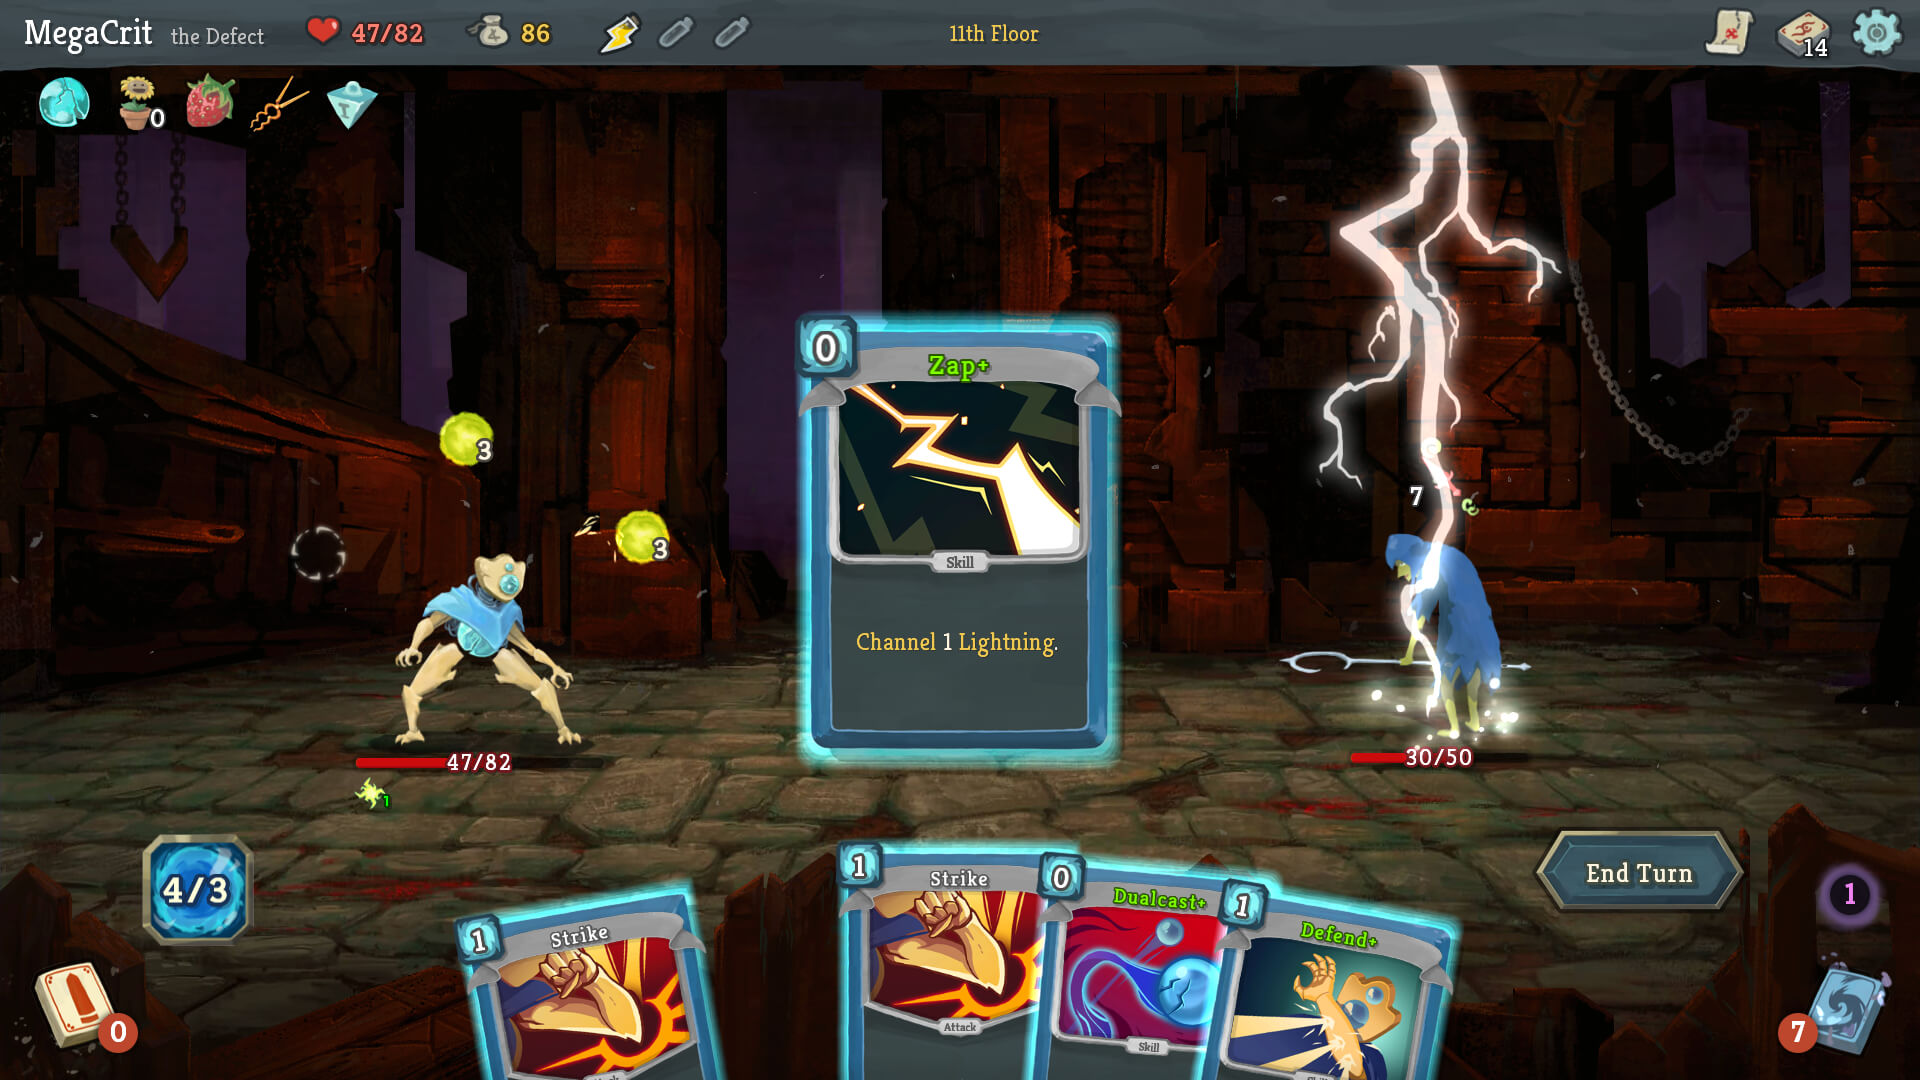
\includegraphics[width=\linewidth]{img/slay_the_spire.jpg}
        \caption{}
        \label{Fig:Style1A}
    \end{subfigure}
    \hfill
    \begin{subfigure}[t]{0.45\linewidth}
        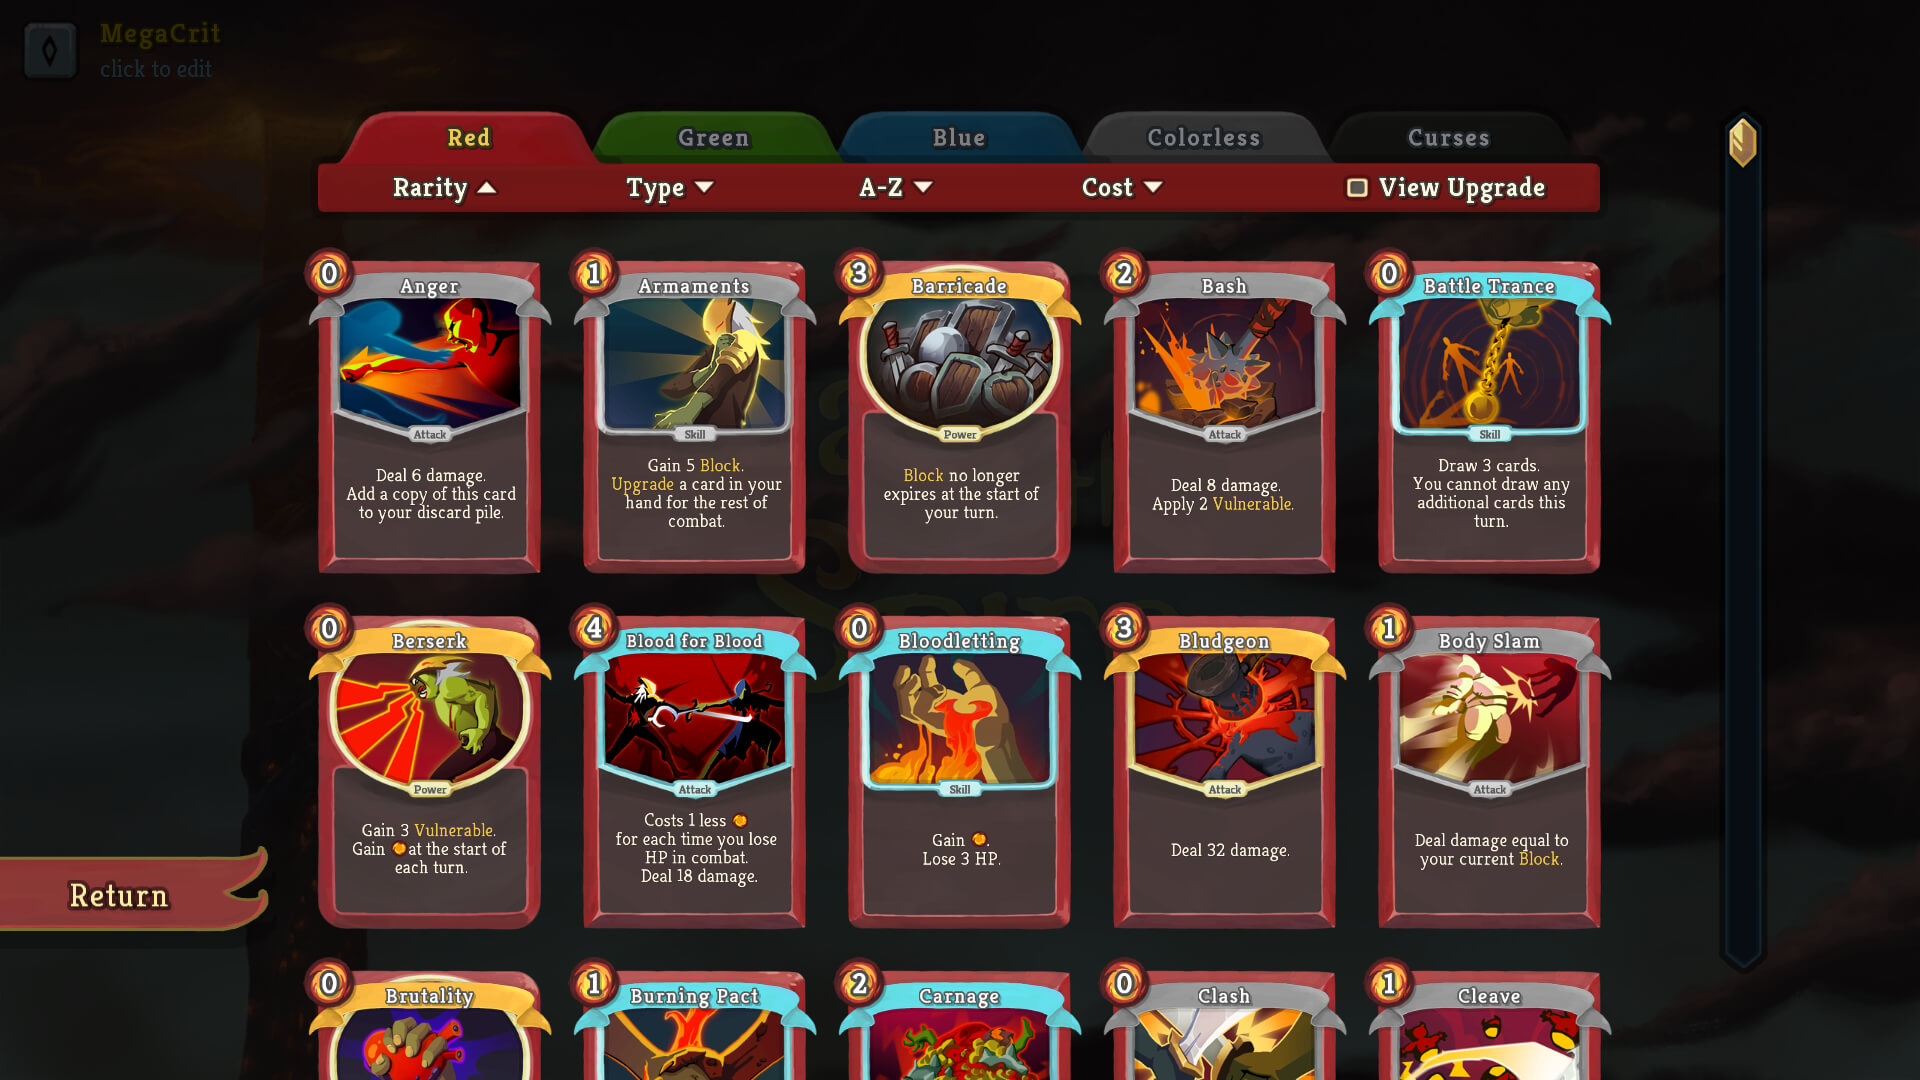
\includegraphics[width=\linewidth]{img/slay_the_spire_2.jpg}
        \caption{}
        \label{Fig:Style1B}
    \end{subfigure}
    \caption{Slay the Spire game screenshots. Retrieved from \cite{slaythespire2024}.}
    \label{Fig:StyleComparison}
\end{figure}


\begin{figure}[h]
    \centering
    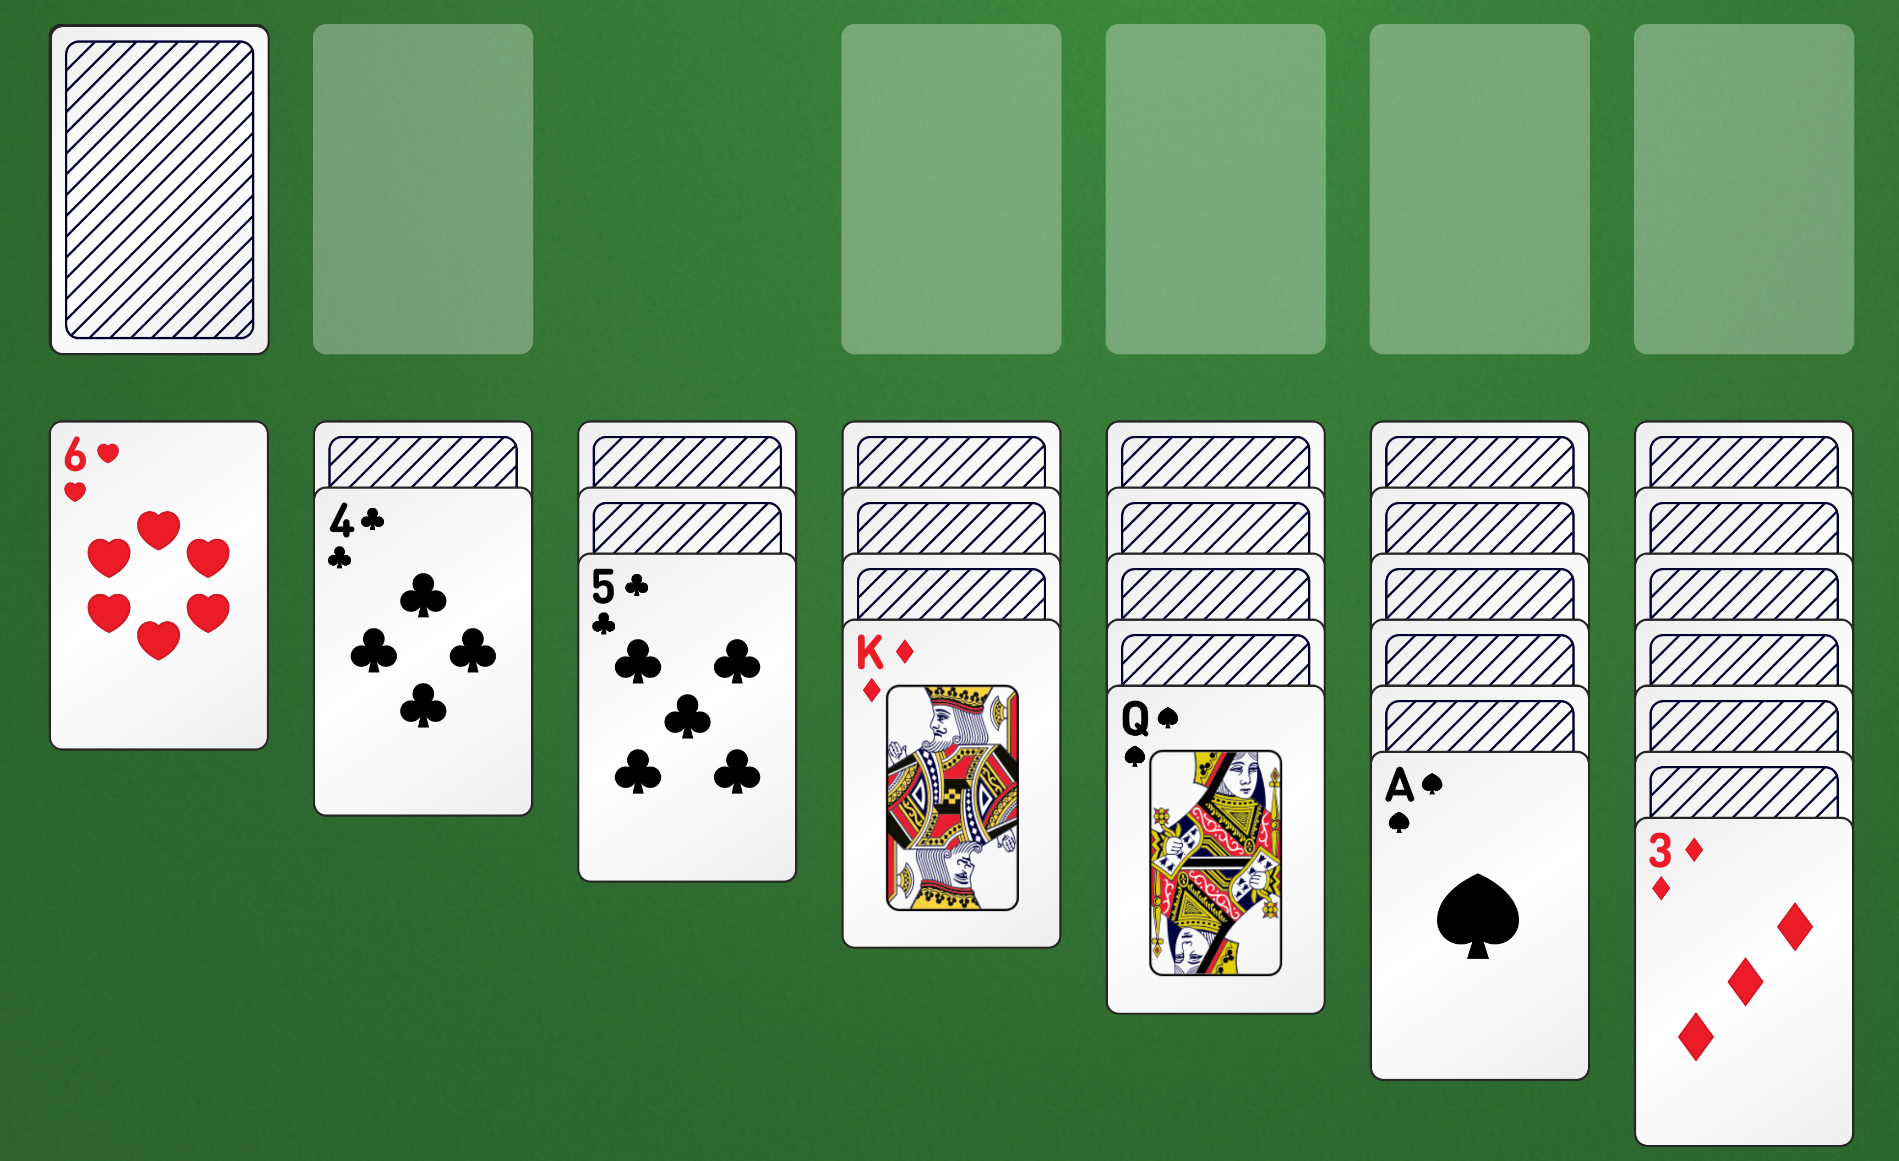
\includegraphics[width=0.5\linewidth]{img/solitaire.png}
    \caption{Classic card game on PC - Solitaire. Retrieved from \cite{goldrushsolitaire2024}.}
    \label{fig:enter-label}
\end{figure}

\begin{figure}[H]
    \centering
    \begin{subfigure}[t]{0.45\linewidth}
        
\includegraphics[width=\linewidth]{img/Balatro_logo.png}
        \caption{}
        \label{Fig:Style1A}
    \end{subfigure}
    \hfill
    \begin{subfigure}[t]{0.45\linewidth}
        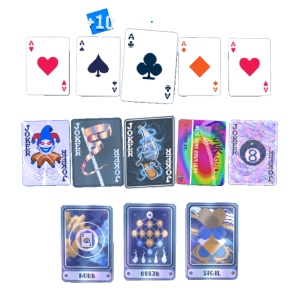
\includegraphics[width=\linewidth]{img/balatro.png}
        \caption{}
        \label{Fig:Style1B}
    \end{subfigure}
    \caption{Balatro logo and card concepts. Retrieved from \cite{balatro2024, balatro_official2024}.}
    \label{Fig:StyleComparison}
\end{figure}

\newpage
\bibliographystyle{czechiso}
\bibliography{bibliography}
\end{document}
